%
% File acl2020.tex
%
%% Based on the style files for ACL 2020, which were
%% Based on the style files for ACL 2018, NAACL 2018/19, which were
%% Based on the style files for ACL-2015, with some improvements
%%  taken from the NAACL-2016 style
%% Based on the style files for ACL-2014, which were, in turn,
%% based on ACL-2013, ACL-2012, ACL-2011, ACL-2010, ACL-IJCNLP-2009,
%% EACL-2009, IJCNLP-2008...
%% Based on the style files for EACL 2006 by 
%%e.agirre@ehu.es or Sergi.Balari@uab.es
%% and that of ACL 08 by Joakim Nivre and Noah Smith

\documentclass[11pt,a4paper]{article}
\usepackage[hyperref]{acl2020}
\usepackage{times}
\usepackage{latexsym}
\renewcommand{\UrlFont}{\ttfamily\small}

% This is not strictly necessary, and may be commented out,
% but it will improve the layout of the manuscript,
% and will typically save some space.
\usepackage{microtype}

\aclfinalcopy % Uncomment this line for the final submission
%\def\aclpaperid{***} %  Enter the acl Paper ID here

%\setlength\titlebox{5cm}
% You can expand the titlebox if you need extra space
% to show all the authors. Please do not make the titlebox
% smaller than 5cm (the original size); we will check this
% in the camera-ready version and ask you to change it back

\usepackage{booktabs}
\usepackage{graphicx}
\graphicspath{{../images/}}

\newcommand\BibTeX{B\textsc{ib}\TeX}

\title{Hyperpartisan News Analysis With Scattertext}

\author{Julen Etxaniz \\
  University of the Basque Country \\
  \texttt{jetxaniz007@ikasle.ehu.eus} \\\And
  Oihane Cantero \\
  University of the Basque Country \\
  \texttt{ocantero003@ikasle.ehu.eus} \\}

\date{}

\begin{document}
\maketitle
\begin{abstract}

\end{abstract}

\section{Introduction}

Hyperpartisan news are those that take an extreme left-wing or right-wing standpoint. Detecting hyperpartisan news automatically can be useful to tag them and inform readers. This was the goal of the SemEval 2019 Task 4 \cite{kiesel2019semeval}.

The purpose of this work is to analyze the usage of words in documents which are hyperpartisan and non-hyperpartisan. Hyperpartisan news are those that exhibit blind, prejudiced, or unreasoning allegiance to one party, faction, cause, or person.

Whereas the task on semeval was to design a system to automatically detect hyperpartisan news, in this exercise we are going to exploit both corpora and analyze which terms are the most relevant in each of the sets.

We use two different methods for analysing hyperpartisan and non-hyperpartisan documents. First, we calculate log-odd ratios to extract the most relevant words of each category. Then, we use Scattertext \cite{kessler2017scattertext} to build an interactive HTML scatter plot. We compare the results of each method and extract some conclusions.

\section{Dataset}

This dataset contains hyperpartisan and non-hyperpartisan news articles published online. The data is divided into two datasets. One has 1,273 articles, each labeled manually, while the second, larger dataset of 754,000 articles is labeled in a semi-automated manner via distant supervision at the publisher level. Each dataset is further divided into training, validation and testing subsets. The articles and ground-truth information of each subset are contained in separate XML files.

The dataset can be downloaded from Zenodo\footnote{\url{https://zenodo.org/record/5776081}}. You can also use the dataset creation script to create a HuggingFace Dataset automatically with the original and cleaned text. It also contains all the metadata attributes that are present in the original files. This could be used to easily build a classifier using the HuggingFace Transformers library.

\subsection{By Publisher Dataset}

The first part of the data is labeled by the overall bias of the publisher as provided by BuzzFeed journalists or \href{https://mediabiasfactcheck.com}{MediaBiasFactCheck.com}. It contains a total of 750,000 articles, half of which (375,000) are hyperpartisan and half of which are not. Half of the articles that are hyperpartisan (187,500) are on the left side of the political spectrum, half are on the right side. 

This data is split into a training set (80\%, 600,000 articles) and a validation set (20\%, 150,000 articles), where no publisher that occurs in the training set also occurs in the validation set. Similarly, none of the publishers in those sets occurs in the test set (4,000 articles).

\subsection{By Article Dataset}

The second part of the data is labeled through crowdsourcing on an article basis. The data contains only articles for which a consensus among the crowdsourcing workers existed. It contains a total of 645 articles. Of these, 238 (37\%) are hyperpartisan and 407 (63\%) are not, We will use a similar balanced test set that contains 628 articles. Again, none of the publishers in this set occurs in the test set.

\section{Methods}

First, we preprocess the original data to get better results in the analysis. Then, we use two different methods for analysing hyperpartisan and non-hyperpartisan documents. On the one hand, we calculate log-odd ratios to extract the most relevant words of each category. On the other hand, we use Scattertext \cite{kessler2017scattertext} to build an interactive HTML scatter plot. Code is available at GitHub: \footnote{\url{https://github.com/juletx/hyperpartisan-news-detection}}

\subsection{Preprocessing}
\label{Preprocessing}
As the original files are XML files, we have to preprocess them in order to obtain good insights. First we use the \texttt{lxml} library in python to analyze the XML documents and extract the necessary information. Preprocessing also includes tokenizing, converting words to lowercase, removing punctuation, numbers, stop words, extra whitespaces, XML entities and image tags.

To calculate the log-odd ratios, we select the validation set of the By Publisher dataset that contains 150,000 articles. The first step is to generate two text files for hyperpartisan and non-hyperpartisan news articles, respectively. We have to divide the news articles contained in the validation XML file, according to their ground truth value.

For scattertext, we select the test set of the By Article Dataset, which contains 628 articles. Scattertext needs a smaller number of articles because otherwise the interactive site takes very long to load. This size is big enough to extract the most relevant words.

\subsection{Log-odd ratio}

After preprocessing text files, we extract the log-odd ratios of each word. Because the log-odd ratio is sensitive to infrequent words, we discard words that appear less than 20 times in the corpus. We also extract the log-odd ratios of the bigrams in the corpus. Having the log-odd ratios, we can extract the most relevant 50 words and bigrams in hyperpartisan and non-hyperpartisan documents. If we analyze these words, we can draw some conclusions about hyperpartisan news.

The log-odd ratio is a measure of words compared on two sets of documents ($i$ and $j$), which in our case corresponds to hyperpartisan and non-hyperpartisan documents, respectively. Each word then can be associated with its log-odd ratio $r_w$, which is a number that can be positive or negative: positive numbers are associated with set $i$, and negative numbers with set $j$.

The log-odd ratio $r_w$ is defined as:
$$p_w^{(i)} = \frac{f_w^{(i)}}{N^{(i)}}; p_w^{(j)} = \frac{f_w^{(j)}}{N^{(j)}}$$
$$o_w^{(i)} = \frac{p_w^{(i)}}{1-p_w^{(i)}}; o_w^{(j)} = \frac{p_w^{(j)}}{1-p_w^{(j)}}$$
$$r_w = \log{o_w^{(i)}} - \log{o_w^{(j)}}$$

where $f_w^{(i)}$ is the frequency of word $w$ in group $i$ (hyperpartisan or non-hyperpartisan), and $N^{(i)}$ is the number of words in group $i$.

\subsection{Scattertext}

Scattertext \cite{kessler2017scattertext} is a tool for finding distinguishing terms in corpora and displaying them in an interactive HTML scatter plot. It is intended for visualizing what words and phrases are more characteristic of a category than others. We can use it to compare hyperpartisan and non-hyperpartisan news. It also gives the terms which occur frequently in all sets of documents being studied (both categories), but relatively infrequent compared to general term frequencies.

Scattertext uses a metric called Scaled F-Score to rank terms. Associated terms have a high category-specific precision and category-specific term frequency. The harmonic mean of precision and frequency is taken to ensure that both are high. Two adjustments are made to come up with the final formulation of Scaled F-Score.

Given a word $w_i \in W$ and a category $c_j \in C$, define the precision of the word $w_i$ with regard to a category as:
$$ \mbox{prec}(i,j) = \frac{\#(w_i, c_j)}{\sum_{c \in C} \#(w_i, c)}. $$

The function $\#(w_i, c_j)$ represents either the number of times $w_i$ occurs in a document labeled with the category $c_j$ or the number of documents labeled $c_j$ which contain $w_i$.

Similarly, define the frequency a word occurs in the category as:
$$ \mbox{freq}(i, j) = \frac{\#(w_i, c_j)}{\sum_{w \in W} \#(w, c_j)}. $$
The harmonic mean of these two values of these two values is defined as:
$$ \mathcal{H}_\beta(i,j) = (1 + \beta^2) \frac{\mbox{prec}(i,j) \cdot \mbox{freq}(i,j)}{\beta^2 \cdot \mbox{prec}(i,j) + \mbox{freq}(i,j)}. $$
$\beta \in \mathcal{R}^+$ is a scaling factor where frequency is favored if $\beta < 1$, precision if $\beta > 1$, and both are equally weighted if $\beta = 1$. F-Score is equivalent to the harmonic mean where $\beta = 1$.

The first problem of the previous formulation is that harmonic means are dominated by precision. To solve this we take the normal CDF of precision and frequency percentage scores, which will be scaled between 0 and 1.

Define the the Normal CDF as:
$$ \Phi(z) = \int_{-\infty}^z \mathcal{N}(x; \mu, \sigma^2)\ \mathrm{d}x.$$

Where $ \mathcal{N} $ is the PDF of the Normal distribution, $\mu$ is the mean, and $\sigma^2$ is the variance. $\Phi$ is used to scale and standardize the precisions and frequencies, and place them on the same scale $[0,1]$.

Now we can define Scaled F-Score as the harmonic mean of the Normal CDF transformed frequency and precision:
$$ \mbox{S-CAT}_{\beta}(i, j) = \mathcal{H}_{\beta}(\Phi(\mbox{prec}(i, j)), \Phi(\mbox{freq}(i, j))).$$
$\mu$ and $\sigma^2$ are defined separately as the mean and variance of precision and frequency.
A $\beta$ of 2 is recommended and is the default value in Scattertext.

Note that any function with the range of $[0,1]$ can be used in place of $\Phi$.  Also, when the precision is very small normalization may be foregone.

The second adjustment consists of making the score fair for negative scoring terms. For this we compute the Scaled F-Score of the negative class. If that score has a higher magnitude than the positive one, we keep that value as a negative score.

Note that the range of $\mathcal{S}$ is now $[-1, 1]$, where $\mathcal{S} < 0$ indicates a term less associated with the category is question than average, and a positive score being more associated.

\section{Results}

The results we get by extracting the words relevant words using log-odd ratios and using Scattertext are different.

\subsection{Using log-odd ratios}

We get relevant words and bigrams from hyperpartisan and non-hyperpartisan articles by calculating their log-odd ratio.

\subsubsection{Relevant Words}

There are many differences betweeen the 50 most relevant words of
hyperpartisan and non-hyperpartisan news. Here are the main findings of each class. Table \ref{tab:words_bigrams} shows all words and bigrams.

\begin{table*}[ht]
\centering
\begin{tabular}{l|l|ll|ll}
\toprule
Hyp Words        & Non Words         & \multicolumn{2}{c}{Hyp Bigrams}  & \multicolumn{2}{c}{Non Bigrams}   \\ \midrule
wonkette          & subsaharan        & repeat      & offenders   & texas         & tribune      \\
vulgarity         & straus            & state       & shall       & may           & subject      \\
realclearpolitics & treasuries        & media       & keep        & emerging      & economies    \\
newsbusters       & zuma              & reserve     & right       & complete      & list         \\
oreilly           & boko              & media       & research    & exchange      & rate         \\
profanity         & tic               & trump       & nt          & us            & assets       \\
kilmeade          & renminbi          & white       & privilege   & texas         & house        \\
vox               & haram             & illegal     & alien       & boko          & haram        \\
chomsky           & bangkok           & like        & college     & emerging      & markets      \\
courteous         & checker           & law         & shall       & dan           & patrick      \\
gofundme          & nigerians         & person      & shall       & southeast     & asian        \\
rcp               & newsom            & legislature & may         & direct        & investment   \\
newsmax           & utaustin          & without     & warning     & sovereign     & wealth       \\
anarchism         & heremore          & threats     & violence    & us            & current      \\
trolling          & tribune           & monday      & friday      & guest         & post         \\
cavuto            & cfr               & agree       & terms       & members       & may          \\
fucking           & custodial         & obama       & nt          & us            & exports      \\
foxnewscom        & myanmar           & us          & maintain    & china         & trade        \\
anarchist         & rakhine           & news        & hour        & growth        & china        \\
susteren          & hun               & bill        & oreilly     & us            & firms        \\
grahamcassidy     & grist             & obamacare   & repeal      & net           & exports      \\
newsletter        & thai              & media       & matters     & research      & associate    \\
chez              & exporters         & news        & team        & exchange      & rates        \\
usmc              & nigeria           & black       & panther     & international & institutions \\
splc              & denuclearization  & hate        & group       & travis        & county       \\
omalley           & crossposted       & independent & journalism  & global        & governance   \\
fuck              & anc               & van         & susteren    & private       & investors    \\
banter            & yen               & false       & flag        & balance       & sheet        \\
madsen            & depreciation      & season      & two         & story         & updated      \\
watters           & rebalance         & research    & team        & jacob         & zuma         \\
beyoncé          & schwarzenegger    & happening   & world       & china         & central      \\
willard           & thailand          & corporate   & media       & china         & government   \\
jerk              & aggregator        & romney      & leads       & east          & north        \\
lgbtq             & sponsors          & officer     & darren      & texas         & austin       \\
globalist         & kyoto             & privately   & owned       & development   & goals        \\
odonnell          & lima              & overdose    & deaths      & suu           & kyi          \\
emmys             & pri               & shall       & made        & think         & worth        \\
mises             & israelpalestinian & darren      & wilson      & advanced      & economies    \\
globalists        & outflow           & big         & league      & bretton       & woods        \\
kliff             & suu               & show        & today       & president     & jacob        \\
individualist     & nigerian          & associate   & editor      & news          & views        \\
fck               & nld               & game        & thrones     & north         & texas        \\
machado           & uschina           & author      & necessarily & texas         & senate       \\
anarchists        & cyberspace        & basic       & income      & states        & china        \\
painkillers       & rebalancing       & ruling      & class       & david         & dewhurst     \\
slager            & inaudible         & divestment  & sanctions   & chinese       & state        \\
shall             & ph                & support     & continue    & think         & china        \\
zionists          & odinga            & america     & health      & southeast     & asia         \\
teabaggers        & bretton           & mr          & comey       & fort          & worth        \\
shep              & hu                & romney      & tax         & african       & national     \\ \bottomrule
\end{tabular}
\caption{Most relevant hyperpartisan and non-hyperpartisan words and bigrams according to log-odd ratios.}
\label{tab:words_bigrams}
\end{table*}

Relevant words of hyperpartisan articles:

\begin{itemize}
\item
  Hyperpartisan articles contain words ending in
  -ist/-ism/-ity(anarchist, anarchism, globalist, globalists,
  individualist, anarchists, zionists, vulgarity, profanity). These do
  not appear in non-hyperpartisan words.
\item
  Other hyperpartisan words that describe people (slager, teabagger,
  shep, lgbtq, courteous). Similar terms do not appear in
  non-hyperpartisan words.
\item
  Bad words in hyperpartisan articles (fucking, trolling, fuck, fck).
  There are no bad words in non-hyperpartisan.
\item
  News sites or webs in hyperpartisan articles (wonkette,
  realclearpolitics, newsbusters, vox, gofundme, newsmax, foxnewscom).
  This suggest that these news sites are commonly associated with
  hyperpartisan news. Most correspond to news agencies in the US. No
  news agencies appear in non-hyperpartisan words.
\item
  Other organizations in hyperpartisan news (usmc (United States Marine
  Corps), splc (Southern Poverty Law Center), emmys). They are US
  organizations.
\item
  People in hyperpartisan articles (oreilly, kilmeade, chomsky, cavuto,
  grahamcassidy, omalley, madsen, beyoncé, willard, odonell, kliff,
  machado, watters, susteren). They correspond to politicians,
  journalists and famous people.
\end{itemize}

Relevant words of non-hyperpartisan articles:

\begin{itemize}
\item
  Demonyms in non-hyperpartisan articles (subsaharan, nigerians, thai,
  israelpalestinian, nigerian). They correspond to people from other
  countries. No demonyms appear in hyperpartisan words.
\item
  Places in non-hyperpartisan articles (bangkok, myanmar, rakhine,
  nigeria, thailand, tribune, kyoto, lima). Many places appear in
  non-hyperpartsan words, none in hyperpartisan words. They correspond
  to other countries and cities.
\item
  People in non-hyperpartisan articles (straus, zuma, newsom, hun,
  schwarzenegger, hu (Hu Jintao)). They correspond to politicians and
  famous people.
\item
  Organizations in non-hyperpartisan articles (treasuries, boko, haram,
  tic, utaustin (The University of Texas at Austin), anc (African
  National Congress, pri (Partido Revolucionario Institucional), nld
  (National League for Democracy)). Unlike hyperpartisan organizations,
  many organizations are from other countries different from the US.
\item
  There are many economics terms in non-hyperpartisan articles
  (renminbi, yen, rebalance, cfr, depreciation, exporters, aggregator,
  outflow). Some correspond to currencies and other to actions or
  people.
\end{itemize}

\subsubsection{Relevant Bigrams}

There are many differences betweeen the 50 most relevant bigrams of
hyperpartisan and non-hyperpartisan news. Here are the main findings of each class. Table \ref{tab:words_bigrams} shows all words and bigrams.

Relevant bigrams of hyperpartisan articles:

\begin{itemize}
\item
  More negative words than on non-hyperpartisan news (threats violence,
  hate group, divestment sanctions, overdose deaths, illegal alien)
\item
  People (obama, trump, bill oreilly, romney, darren wilson, mr comey,
  van susteren). They correspond to politicians or famous people
\item
  Media related terms (media research, independent journalism, media
  matters, corporate media, associate editor)
\item
  Politics related terms (trump obama, legislature, obamacare, america
  health, basic income, ruling class)
\end{itemize}

Relevant bigrams of non-hyperpartisan articles:

\begin{itemize}
\item
  Demonyms in non-hyperpartisan articles (southeast asian, african).
\item
  Places in non-hyperpartisan news (texas, us, china, southeast asia,
  travis county, austin). Some places are repeated a lot in different
  bigrams: china, us and texas are the most repeated ones.
\item
  Many economics related bigrams also appear a lot (emerging economies,
  exchange rate, emerging markets, direct investment, private
  investors\ldots).
\item
  Organizations (boko haram, international institutions, china
  gorvernment\ldots)
\item
  People are also mentioned (dan patrick, jacob zuma, suu kyi, president
  jacob, david dewhurst)
\end{itemize}

\subsection{Scattertext}

We visualized the differences between hyperpartisan and non-hyperpartisan of the original text and cleaned text (before and after the preprocessing of the text mentionned in section \ref{Preprocessing}).

\subsubsection{Original text}

Most frequent words in both hyperpartisan articles are stopwords, and we can also see that in both cases some there are some non-words character sequences (= twsrc\%5etfw, type="external">august). We can see all the words and which of them appear most in hyperpartisan and non-hyperpartisan articles in Figure \ref{fig:byarticle_test}. 

\begin{figure*}[ht]
    \centering
    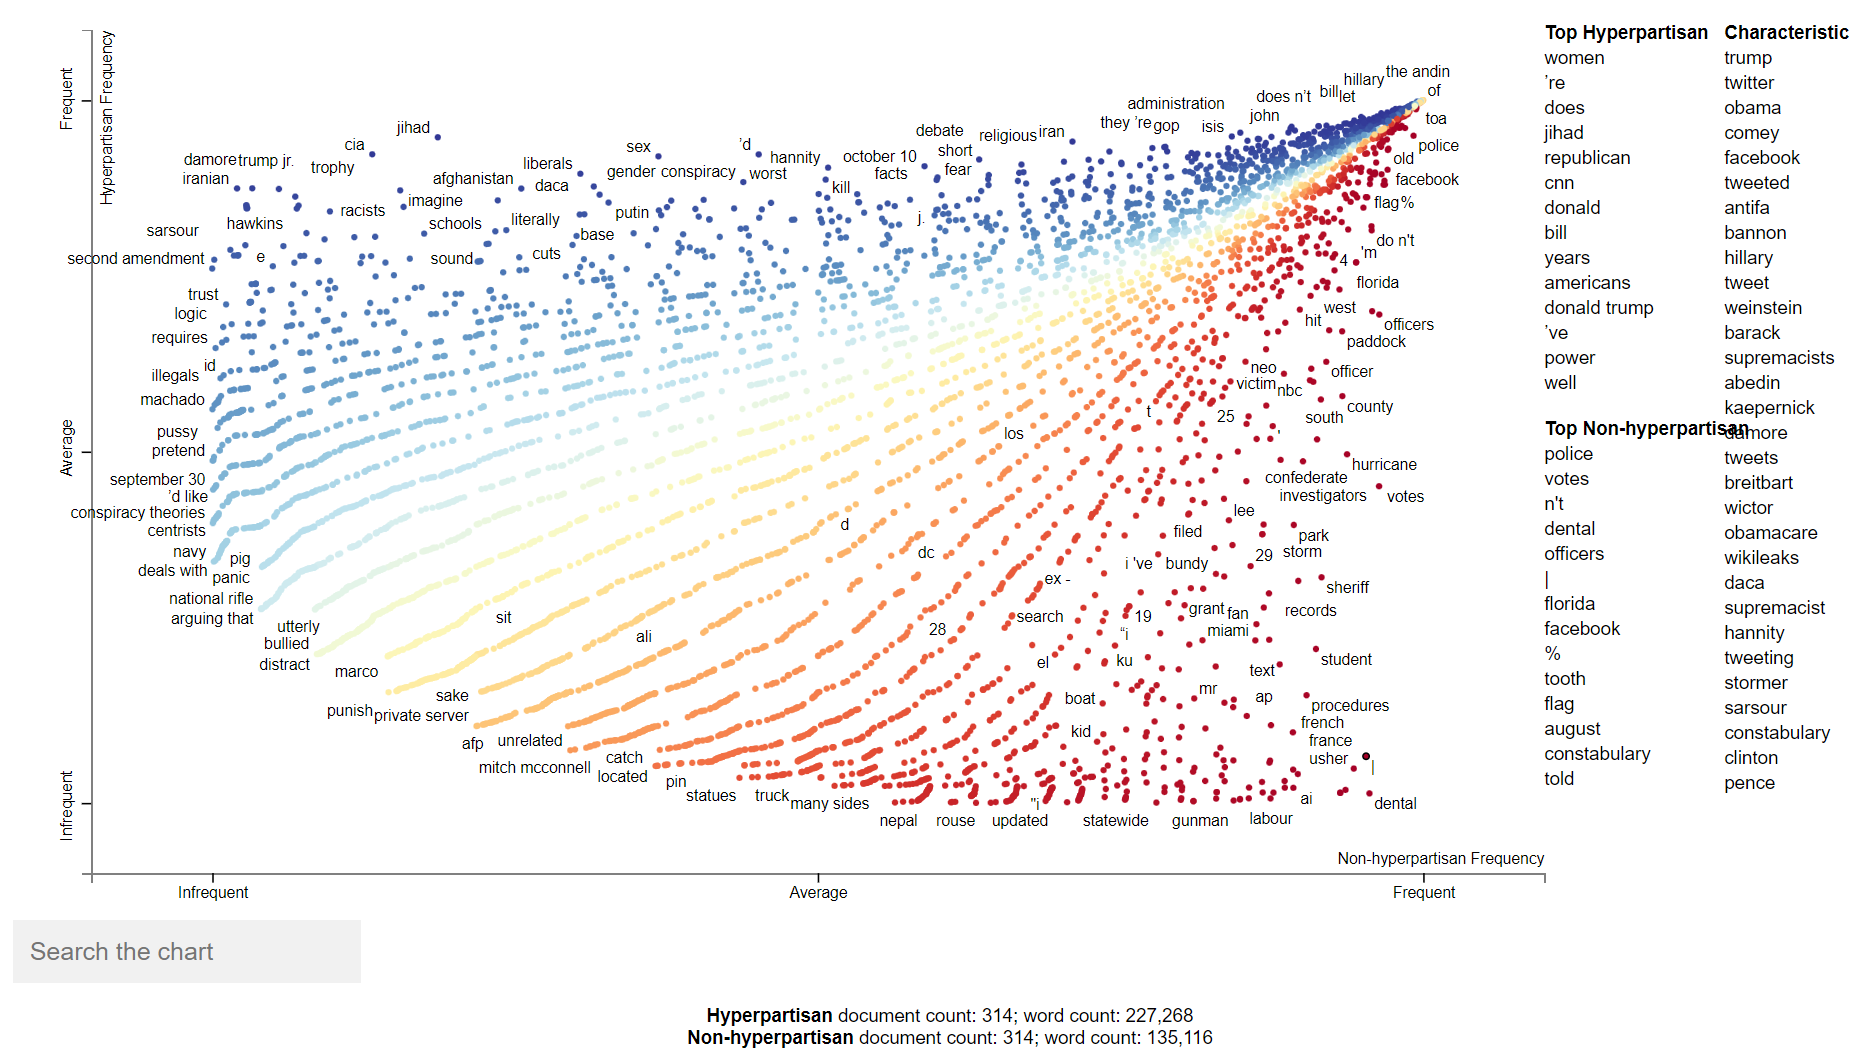
\includegraphics[width=\linewidth]{byarticle_test.png}
    \caption{Scattertext plot and top words for the original test set of the By Article dataset.}
    \label{fig:byarticle_test}
\end{figure*}

\begin{figure*}[ht]
    \centering
    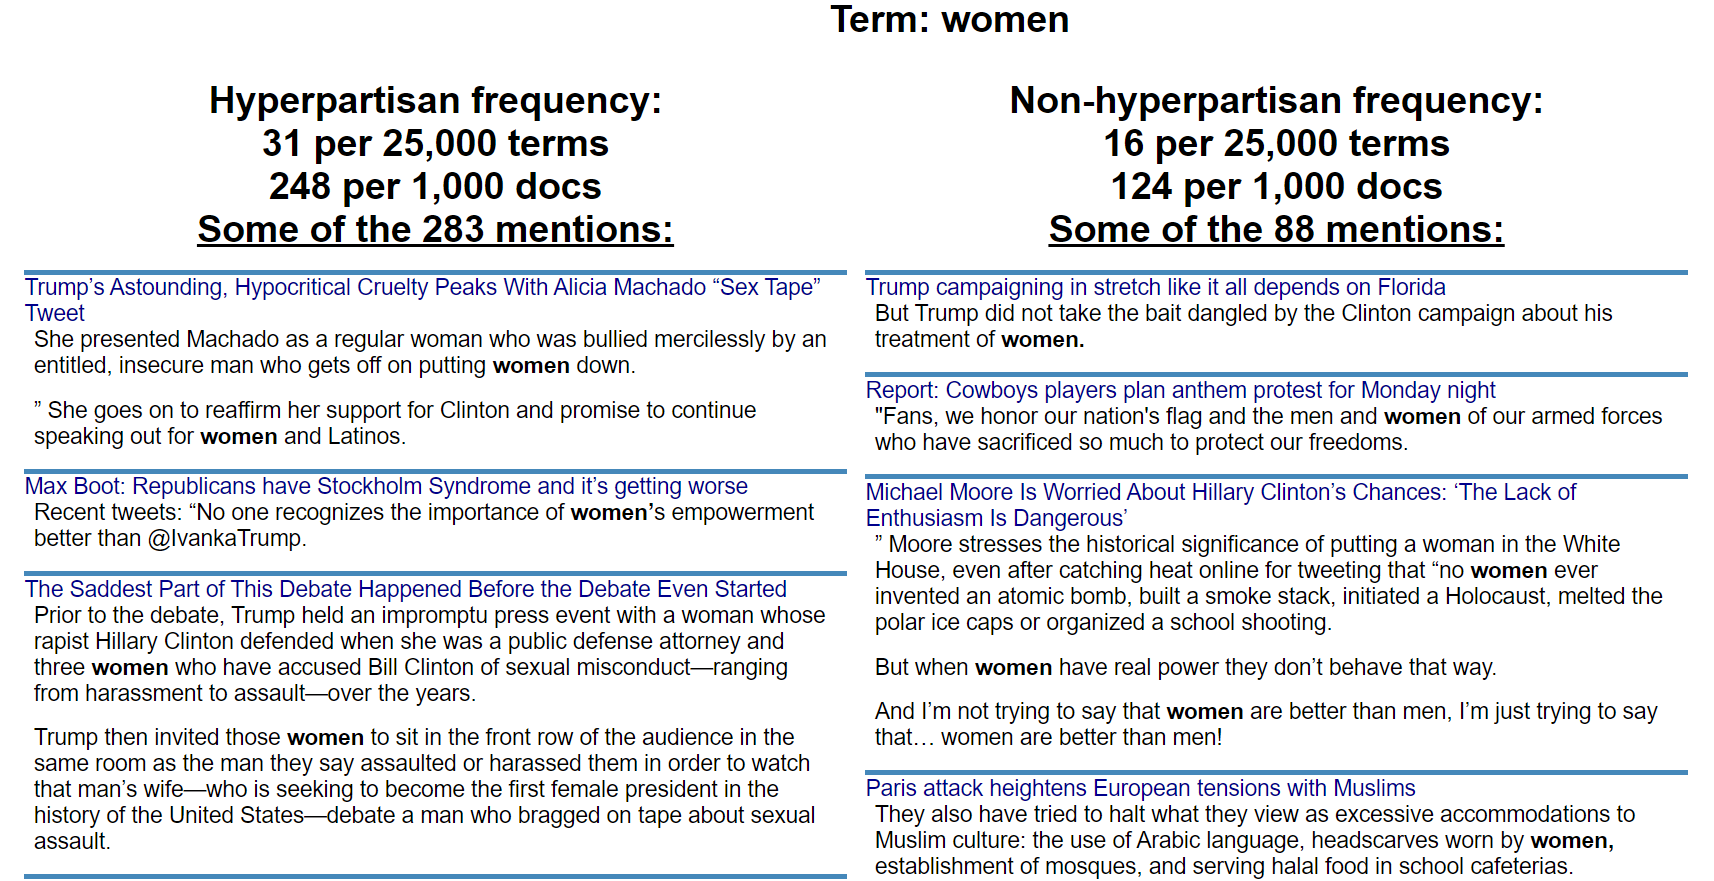
\includegraphics[width=\linewidth]{byarticle_test_search.png}
    \caption{Scattertext search example of the term women in hyperpartisan and non-hyperpartisan documents.}
    \label{fig:byarticle_test_search}
\end{figure*}

Relevant words of hyperpartisan articles:

\begin{itemize}
    \item Names of people and words of the political domain (donald trump, politics, republican, second amendment)
    \item Names of countries (iranian, afghanistan)
    \item Stopwords (it's, he's, does, that's)
\end{itemize}

Relevant words of non-hyperpartisan articles:

\begin{itemize}
    \item Words that doesn't seem to have any political connotation (dental, tooth, tooth regeneration). These words probably appear in the same articles, because they are all from the same field
    \item Characters that don't form words (", | a, |)
\end{itemize}

Overall we see that this corpus needs to be cleaned, as there are a lot of stopwords and character sequences that doesn't form words (from URLs, for example). 

\subsubsection{Clean text}
By cleaning the text, we get better results, as the all the words we get for both top-hyperpartisan and non-hyperpartisan terms exists. We can see all the words and which of them appear most in hyperpartisan and non-hyperpartisan articles in Figure \ref{fig:byarticle_test_clean}.
 
\begin{figure*}[ht]
    \centering
    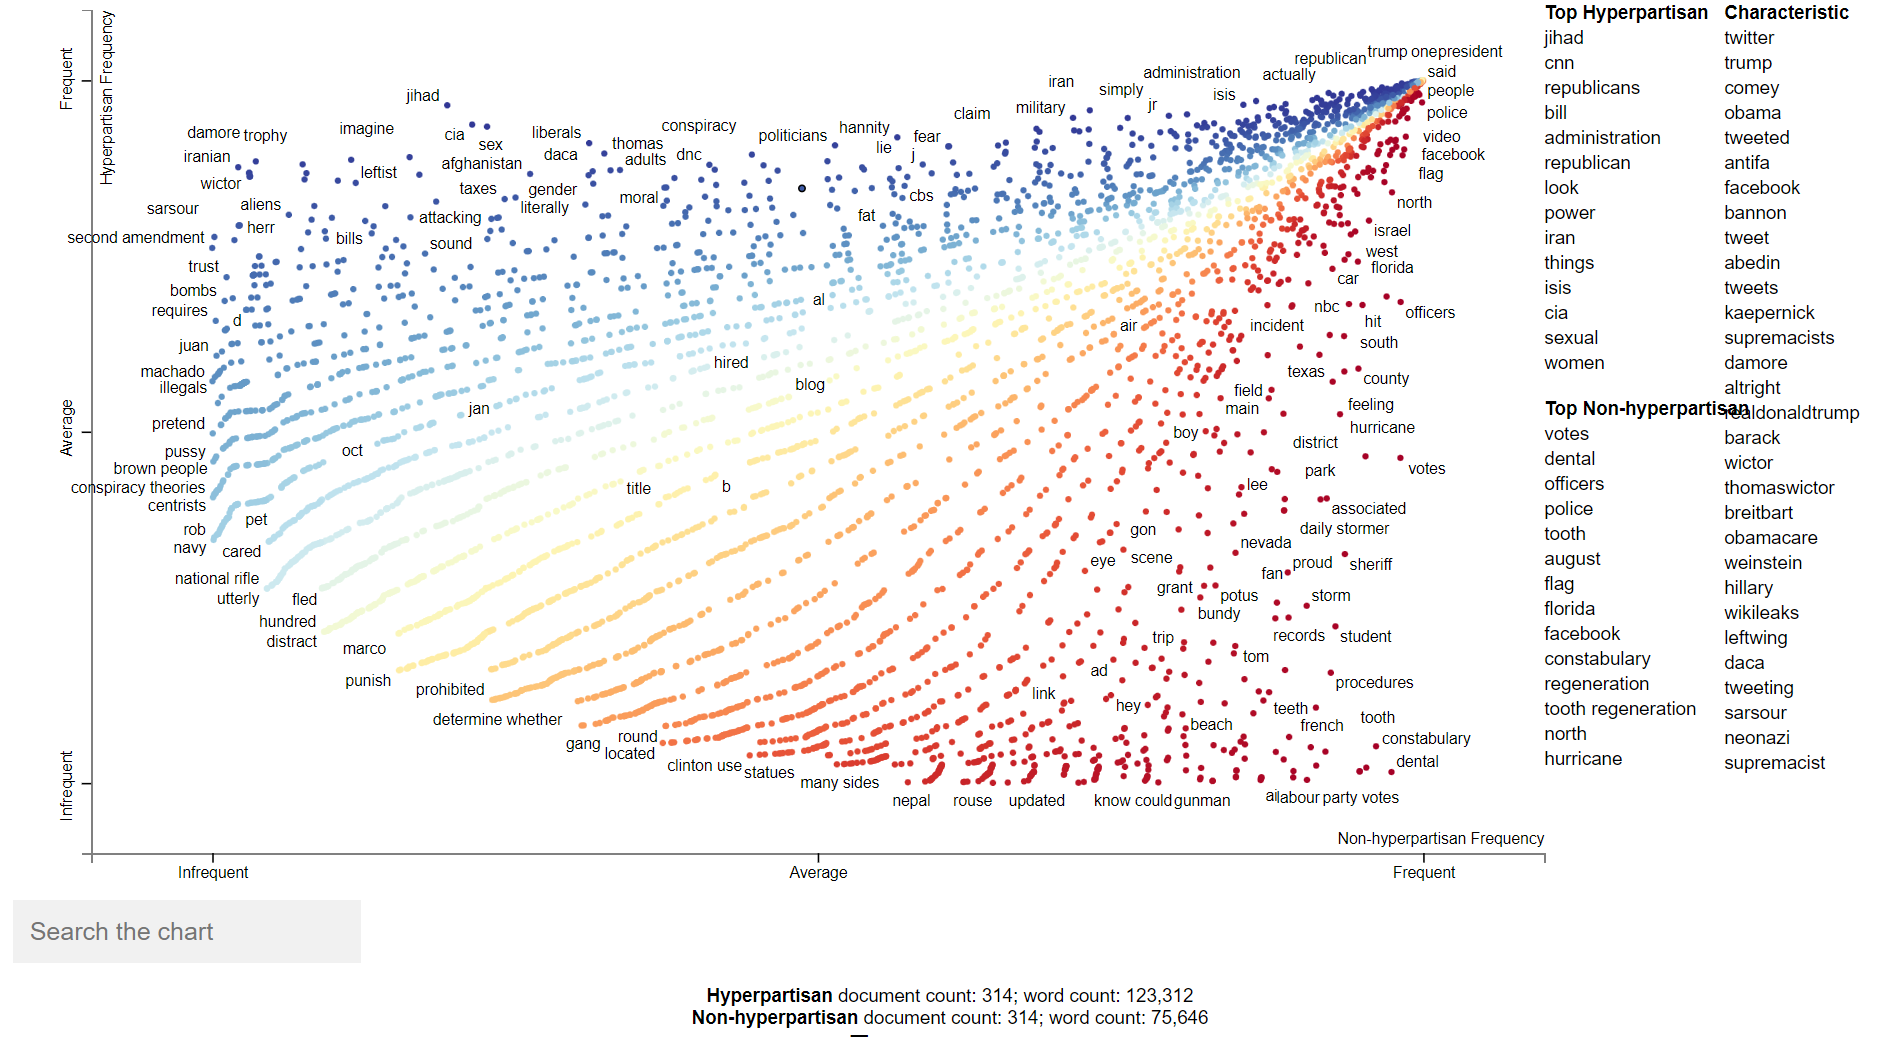
\includegraphics[width=\linewidth]{byarticle_test_clean.png}
    \caption{Scattertext plot and top words for the cleaned test set of the By Article dataset.}
    \label{fig:byarticle_test_clean}
\end{figure*}

Relevant words of hyperpartisan articles:

\begin{itemize}
    \item Words related to politics and organizations (republican, cia, isis, jihad)
    \item People's names (damore, wictor) 
    \item Names of countries (iranian, afghanistan)
\end{itemize}


Relevant words of non-hyperpartisan articles:

\begin{itemize}
    \item Words related to the institutions (votes, flag, police, officers, constabulary)
    \item As in the original text, words that doesn't seem to have any political connotation (dental, tooth, tooth regeneration, august)
\end{itemize}

If we compare the results of Figures \ref{fig:byarticle_test} and \ref{fig:byarticle_test_clean}), we can see that words from the cleaned corpus also appear in the original ones, and for most of them in the same place. And if we look at the more characteristic words of the whole corpus, we see that they are almost the same, and they usually have political connotation (trump, obama, antifa, supremacist, neonazi...).

\section{Conclusions}

We saw that with both methods, we got similar results, we find almost the same words classified as hyperpartisan and non-hyperpartisan, but the visualization with Scattertext makes the results more readable. 

\bibliography{hyperpartisan_news_detection}
\bibliographystyle{acl_natbib}

\end{document}
